% =====================================================================
% Presentación: Detección de fraude en transacciones financieras
% Compilar con: pdflatex presentacion.tex
% (o latexmk -pdf presentacion.tex)
%
% Estructura principal: 12 diapositivas (11 de contenido + cierre).
% El apéndice contiene tablas extensas, figuras y respuestas de respaldo.
% =====================================================================

\documentclass[aspectratio=169,11pt]{beamer}

% ------------------------- Paquetes -----------------------------------
\usepackage[utf8]{inputenc}
\usepackage[T1]{fontenc}
\usepackage[spanish]{babel}
\usepackage{lmodern}
\usepackage{amsmath,amssymb}
\usepackage{booktabs}
\usepackage{graphicx}
\usepackage{array}
\usepackage{multirow}
\usepackage{ragged2e}

% ------------------------- Tema ---------------------------------------
\usetheme{Madrid}
\usecolortheme{whale}
\setbeamertemplate{navigation symbols}{}
\setbeamertemplate{footline}[frame number]
\setbeamerfont{title}{size=\LARGE,series=\bfseries}
\setbeamerfont{frametitle}{size=\large,series=\bfseries}

% ------------------------- Datos --------------------------------------
\title[Detección de fraude]{Detección de Fraude en Transacciones Financieras}
\subtitle{Comparación de clasificadores supervisados}
% Reemplazar [Integrante 2] por el nombre real antes de la entrega.
\author{Oscar y [Integrante 2]}
\institute{Inteligencia Artificial --- Cuarto curso}
\date{Octubre de 2026}

\begin{document}

% =====================================================================
% 1. PORTADA Y OBJETIVO
% =====================================================================
\begin{frame}[t]
  \begin{center}
    {\LARGE\bfseries Detección de Fraude en Transacciones Financieras}\\[0.2cm]
    {\large Comparación de clasificadores supervisados}\\[0.35cm]
    {\normalsize Integrantes: Oscar \quad \textbullet \quad [Integrante 2]}\\[0.12cm]
    {\small Inteligencia Artificial --- Cuarto curso \quad | \quad Octubre de 2026}
  \end{center}

  \vspace{0.25cm}
  \begin{block}{Objetivo}
    \small
    Comparar \textbf{k-NN}, \textbf{Árbol de Decisión}, \textbf{SVM lineal} y un
    \textbf{Random Forest propio} para detectar fraude, priorizando la
    \textbf{minimización de falsos negativos} (maximizar el Recall). La
    Precisión se usa como criterio secundario de desempate.
  \end{block}

  \vspace{0.1cm}
  \begin{itemize}
    \small
    \item 8 configuraciones experimentales: 4 modelos \(\times\) con/sin
          compensación del desbalance.
    \item Pipeline reproducible, modular y libre de \textit{data leakage}.
    \item Evaluación final sobre un 30\,\% de prueba congelado.
  \end{itemize}
\end{frame}

% =====================================================================
% 2. EXPLORACIÓN DE LOS DATOS
% =====================================================================
\section{Objetivo y datos}

\begin{frame}{Exploración de los datos}
  \begin{columns}[T]
    \begin{column}{0.48\textwidth}
      \begin{block}{Dataset completo}
        \scriptsize
        \begin{tabular}{@{}lr@{}}
          \toprule
          Transacciones & 284.807 \\
          Variables & 30 \\
          Legítimas (0) & 284.315 (99,828\,\%) \\
          Fraudes (1) & 492 (0,172\,\%) \\
          Desbalance & 1 : 578 \\
          Duplicados & 1.081 \\
          Valores nulos & 0 \\
          \bottomrule
        \end{tabular}
      \end{block}
    \end{column}
    \begin{column}{0.48\textwidth}
      \begin{block}{Muestra de trabajo}
        \scriptsize
        \begin{tabular}{@{}lr@{}}
          \toprule
          Transacciones & 50.000 \\
          Fraudes & 86 (0,172\,\%) \\
          Train / Test & 35.000 / 15.000 \\
          Fraudes en test & 26 \\
          \bottomrule
        \end{tabular}
      \end{block}
      \vspace{0.1cm}
      {\scriptsize Dataset público \textit{Credit Card Fraud Detection}.
      Submuestra estratificada por coste computacional; el pipeline
      admite el dataset completo.}
    \end{column}
  \end{columns}

  \vspace{0.12cm}
  \begin{block}{Desafíos}
    \scriptsize
    \begin{itemize}
      \item Desbalance extremo: la clase mayoritaria domina cualquier
            métrica global.
      \item Variables \texttt{V1}--\texttt{V28} anonimizadas por PCA;
            \texttt{Time} y \texttt{Amount} en escalas muy distintas.
      \item Solo dos días de transacciones y orden temporal: el split
            aleatorio puede mezclar periodos.
      \item La exactitud es engañosa: predecir siempre legítimo da
            99,83\,\% de exactitud y 0\,\% de Recall.
    \end{itemize}
  \end{block}
\end{frame}

% =====================================================================
% 3. METODOLOGÍA I
% =====================================================================
\section{Metodología}

\begin{frame}{Metodología I: flujo y prevención de fuga}
  \begin{block}{Flujo del experimento}
    \small
    \centering
    \texttt{Datos} $\to$ \texttt{Split 70/30} $\to$ \texttt{CV=5}\\
    $\downarrow$\\
    \texttt{Scaler} $\to$ \texttt{SelectKBest} $\to$ \texttt{Resampler}
    $\to$ \texttt{Modelo} $\to$ \texttt{Test congelado}
  \end{block}

  \begin{columns}[T]
    \begin{column}{0.48\textwidth}
      \begin{block}{Procedimiento}
        \scriptsize
        \begin{enumerate}
          \item División estratificada 70/30 con semilla 42; test reservado.
          \item \texttt{StratifiedKFold(5)} sobre el 70\,\% de entrenamiento.
          \item \texttt{RandomizedSearchCV}: Recall principal, Precisión
                como desempate.
          \item Reentrenamiento sobre todo el 70\,\% y evaluación única en test.
        \end{enumerate}
      \end{block}
    \end{column}
    \begin{column}{0.48\textwidth}
      \begin{block}{Anti-\textit{data leakage}}
        \scriptsize
        \begin{itemize}
          \item \texttt{imblearn.pipeline.Pipeline}: el remuestreador solo
                actúa durante \texttt{fit}.
          \item Escalado y selección se ajustan únicamente con el fold de
                entrenamiento.
          \item El fold de validación y el 30\,\% de prueba nunca se
                remuestrean.
          \item El test no participa en selección, ajuste ni umbral.
        \end{itemize}
      \end{block}
    \end{column}
  \end{columns}

  \vspace{0.1cm}
  \begin{alertblock}{Por qué importa}
    \small
    Si el escalado o el remuestreo se ajustaran con todo el dataset, la
    evaluación estaría contaminada y el rendimiento en producción sería menor.
  \end{alertblock}
\end{frame}

% =====================================================================
% 4. METODOLOGÍA II
% =====================================================================
\begin{frame}{Metodología II: matriz experimental}
  \scriptsize
  \setlength{\tabcolsep}{3pt}
  \renewcommand{\arraystretch}{1.1}
  \resizebox{\textwidth}{!}{%
  \begin{tabular}{@{}llll@{}}
    \toprule
    \textbf{ID} & \textbf{Clasificador} & \textbf{Compensación} & \textbf{Pipeline} \\
    \midrule
    EXP\_1 & k-NN        & No & Scaler + Selección + k-NN \\
    EXP\_2 & k-NN        & Sí & Scaler + Selección + Under + k-NN \\
    EXP\_3 & Árbol       & No & Selección + Árbol \\
    EXP\_4 & Árbol       & Sí & Selección + Under + Árbol \\
    EXP\_5 & SVM lineal  & No & Scaler + Selección + SVM \\
    EXP\_6 & SVM lineal  & Sí & Scaler + Selección + Under + SVM \\
    EXP\_7 & RF propio   & No & Selección + CustomRandomForest \\
    EXP\_8 & RF propio   & Sí & Selección + Under + CustomRandomForest \\
    \bottomrule
  \end{tabular}%
  }

  \vspace{0.15cm}
  \begin{columns}[T]
    \begin{column}{0.49\textwidth}
      \begin{block}{Preprocesamiento}
        \scriptsize
        \begin{itemize}
          \item \texttt{StandardScaler} solo para k-NN y SVM.
          \item \texttt{SelectKBest} con \texttt{f\_classif}; información
                mutua disponible.
          \item \(k \in \{10,20,\text{todas}\}\).
          \item \texttt{RandomUnderSampler} por defecto; \texttt{SMOTE}
                como alternativa.
        \end{itemize}
      \end{block}
    \end{column}
    \begin{column}{0.49\textwidth}
      \begin{block}{Métricas}
        \scriptsize
        \begin{itemize}
          \item Recall (sensibilidad) y FNR.
          \item Precisión, especificidad, F1 y exactitud.
          \item Matriz de confusión y reportes automáticos.
          \item Selección por Recall; Precisión como desempate.
        \end{itemize}
      \end{block}
    \end{column}
  \end{columns}
\end{frame}

% =====================================================================
% 5. RANDOM FOREST PROPIO: DISEÑO
% =====================================================================
\section{Random Forest propio}

\begin{frame}{Random Forest propio: diseño}
  \begin{columns}[T]
    \begin{column}{0.49\textwidth}
      \begin{block}{Construcción}
        \scriptsize
        \begin{itemize}
          \item Hereda de \texttt{BaseEstimator} y \texttt{ClassifierMixin}.
          \item \(T\) árboles; cada uno entrena con una muestra bootstrap
                de tamaño \(N\) con reemplazo.
          \item Subespacio aleatorio: cada división considera solo
                \texttt{max\_features} variables.
          \item Semillas independientes derivadas de la semilla global.
          \item Sin \texttt{RandomForestClassifier} ni
                \texttt{BaggingClassifier}.
        \end{itemize}
      \end{block}
    \end{column}
    \begin{column}{0.49\textwidth}
      \begin{block}{Predicción}
        \scriptsize
        \begin{itemize}
          \item Votación mayoritaria de los \(T\) árboles.
          \item Empate: se prioriza la clase positiva (fraude).
          \item \texttt{predict\_proba}: promedio de probabilidades.
          \item Parámetros: \texttt{n\_estimators}, \texttt{max\_depth},
                \texttt{max\_features}, \texttt{min\_samples\_leaf},
                \texttt{random\_state}.
        \end{itemize}
      \end{block}
    \end{column}
  \end{columns}

  \vspace{0.15cm}
  \begin{block}{Papel del bagging y del subespacio aleatorio}
    \small
    El bagging reduce la varianza al promediar árboles diversos; el
    subespacio aleatorio decorrelaciona los árboles y evita que una sola
    variable domine. Juntos mejoran la estabilidad y la generalización
    frente a un árbol único.
  \end{block}
\end{frame}

% =====================================================================
% 6. RANDOM FOREST PROPIO: PSEUDOCÓDIGO
% =====================================================================
\begin{frame}{Random Forest propio: pseudocódigo}
  \begin{columns}[T]
    \begin{column}{0.58\textwidth}
      \begin{block}{Algoritmo}
        \ttfamily\scriptsize
        for $t = 1,\dots,T$:\\
        \hspace*{0.4cm}seed$_t$ $\leftarrow$ derive(random\_state)\\
        \hspace*{0.4cm}idx$_t$ $\leftarrow$ bootstrap($N$, replace=True)\\
        \hspace*{0.4cm}tree$_t$ $\leftarrow$ DecisionTree(max\_depth, max\_features, ...)\\
        \hspace*{0.4cm}tree$_t$.fit($X$[idx$_t$], $y$[idx$_t$])\\[2pt]
        predict($x$):\\
        \hspace*{0.4cm}votes $\leftarrow$ [tree$_t$.predict($x$) for $t=1,\dots,T$]\\
        \hspace*{0.4cm}return majority\_vote(votes) \# empate $\to$ clase 1
      \end{block}
    \end{column}
    \begin{column}{0.39\textwidth}
      \begin{block}{Parámetros configurables}
        \scriptsize
        \begin{tabular}{@{}ll@{}}
          \toprule
          Parámetro & Valores \\
          \midrule
          \texttt{n\_estimators} & 50, 100 \\
          \texttt{max\_depth} & None, 10, 20 \\
          \texttt{max\_features} & sqrt, log2 \\
          \texttt{min\_samples\_leaf} & 1, 5 \\
          \texttt{random\_state} & 42 \\
          \bottomrule
        \end{tabular}
      \end{block}
      \vspace{0.1cm}
      {\scriptsize Cada árbol es un \texttt{DecisionTreeClassifier};
      el bosque se construye en \texttt{CustomRandomForest.fit}.}
    \end{column}
  \end{columns}
\end{frame}

% =====================================================================
% 7. SELECCIÓN DE HIPERPARÁMETROS
% =====================================================================
\section{Selección de hiperparámetros}

\begin{frame}{Selección de hiperparámetros}
  \scriptsize
  \setlength{\tabcolsep}{2.5pt}
  \renewcommand{\arraystretch}{1.1}
  \resizebox{\textwidth}{!}{%
  \begin{tabular}{@{}l p{4.2cm} p{4.8cm} c@{}}
    \toprule
    \textbf{ID} & \textbf{Espacio explorado} & \textbf{Configuración seleccionada} & \textbf{CV Recall} \\
    \midrule
    EXP\_1 & \(k\in\{3,5,7,11\}\); pesos; \(k_f\)
           & \(k=11\), distance, \(k_f=10\) & \(0.850 \pm 0.122\) \\
    EXP\_2 & ídem EXP\_1
           & \(k=3\), uniform, \(k_f=10\) & \(0.900 \pm 0.062\) \\
    EXP\_3 & prof.\ \(\{None,5,10,20\}\); hoja \(\{1,5,20\}\); criterio; \(k_f\)
           & prof.\ 20, hoja 20, gini, \(k_f=20\) & \(0.733 \pm 0.097\) \\
    EXP\_4 & ídem EXP\_3
           & prof.\ 5, hoja 1, gini, \(k_f=20\) & \(0.900 \pm 0.122\) \\
    EXP\_5 & \(C\in\{0.01,0.1,1,10\}\); \(k_f\)
           & \(C=10\), \(k_f=20\) & \(0.750 \pm 0.075\) \\
    EXP\_6 & ídem EXP\_5
           & \(C=0.1\), \(k_f=\text{all}\) & \textbf{\(0.950 \pm 0.041\)} \\
    EXP\_7 & \(T\in\{50,100\}\); prof.; max\_features; hoja; \(k_f\)
           & \(T=100\), prof.\ 10, hoja 1, sqrt, \(k_f=20\) & \(0.767 \pm 0.097\) \\
    EXP\_8 & ídem EXP\_7
           & \(T=50\), prof.\ libre, hoja 1, sqrt, \(k_f=10\) & \(0.917 \pm 0.053\) \\
    \bottomrule
  \end{tabular}%
  }
  \vspace{0.12cm}
  \footnotesize
  \textbf{CV Recall}: media \(\pm\) desviación estándar en
  \texttt{StratifiedKFold(5)}. Criterio: mayor Recall medio; Precisión
  media como desempate. \texttt{RandomizedSearchCV} evalúa 8--12
  candidatos por experimento. \(k_f\): n.º de variables; prof.:
  profundidad; \(T\): n.º de árboles; pesos: uniform/distance;
  criterio: gini/entropy; \texttt{max\_features}: sqrt/log2.
\end{frame}

% =====================================================================
% 8. RESULTADOS EN PRUEBA I
% =====================================================================
\section{Resultados}

\begin{frame}{Resultados en prueba: sin y con compensación}
  \scriptsize
  \setlength{\tabcolsep}{2.5pt}
  \renewcommand{\arraystretch}{1.1}
  \resizebox{\textwidth}{!}{%
  \begin{tabular}{@{}l l c c c c c c c@{}}
    \toprule
    \textbf{ID} & \textbf{Modelo} & \textbf{Comp.} &
    \textbf{Recall} & \textbf{Prec.} & \textbf{Espec.} &
    \textbf{F1} & \textbf{Exact.} & \textbf{FNR} \\
    \midrule
    EXP\_1 & k-NN       & No & 0.808 & \textbf{0.875} & 0.9998 & \textbf{0.840} & 0.9995 & 0.192 \\
    EXP\_2 & k-NN       & Sí & \textbf{0.923} & 0.068 & 0.9780 & 0.126 & 0.9779 & \textbf{0.077} \\
    EXP\_3 & Árbol      & No & 0.731 & 0.760 & 0.9996 & 0.745 & 0.9991 & 0.269 \\
    EXP\_4 & Árbol      & Sí & 0.808 & 0.013 & 0.8898 & 0.025 & 0.8897 & 0.192 \\
    EXP\_5 & SVM        & No & 0.769 & 0.800 & 0.9997 & 0.784 & 0.9993 & 0.231 \\
    EXP\_6 & SVM        & Sí & \textbf{0.923} & 0.011 & 0.8577 & 0.022 & 0.8578 & \textbf{0.077} \\
    EXP\_7 & RF propio  & No & 0.769 & 0.870 & 0.9998 & 0.816 & 0.9994 & 0.231 \\
    EXP\_8 & RF propio  & Sí & 0.885 & 0.035 & 0.9580 & 0.068 & 0.9579 & 0.115 \\
    \bottomrule
  \end{tabular}%
  }

  \vspace{0.12cm}
  \begin{block}{Hallazgos}
    \scriptsize
    \begin{itemize}
      \item Sin compensación: EXP\_1 logra el mejor equilibrio
            (Precisión 0.875, F1 0.840); el RF supera al árbol
            (F1 0.816 frente a 0.745).
      \item Con compensación: el Recall sube a 0.923 (EXP\_2/EXP\_6),
            pero la Precisión cae a 0.068/0.011 y los FP pasan a
            330/2.131.
      \item EXP\_8 (RF + under): 0.885 de Recall, 0.035 de Precisión,
            0.068 de F1 y 629 FP.
    \end{itemize}
  \end{block}
\end{frame}

% =====================================================================
% 9. RESULTADOS EN PRUEBA II
% =====================================================================
\begin{frame}{Resultados en prueba: lectura visual}
  \begin{columns}[T]
    \begin{column}{0.62\textwidth}
      \centering
      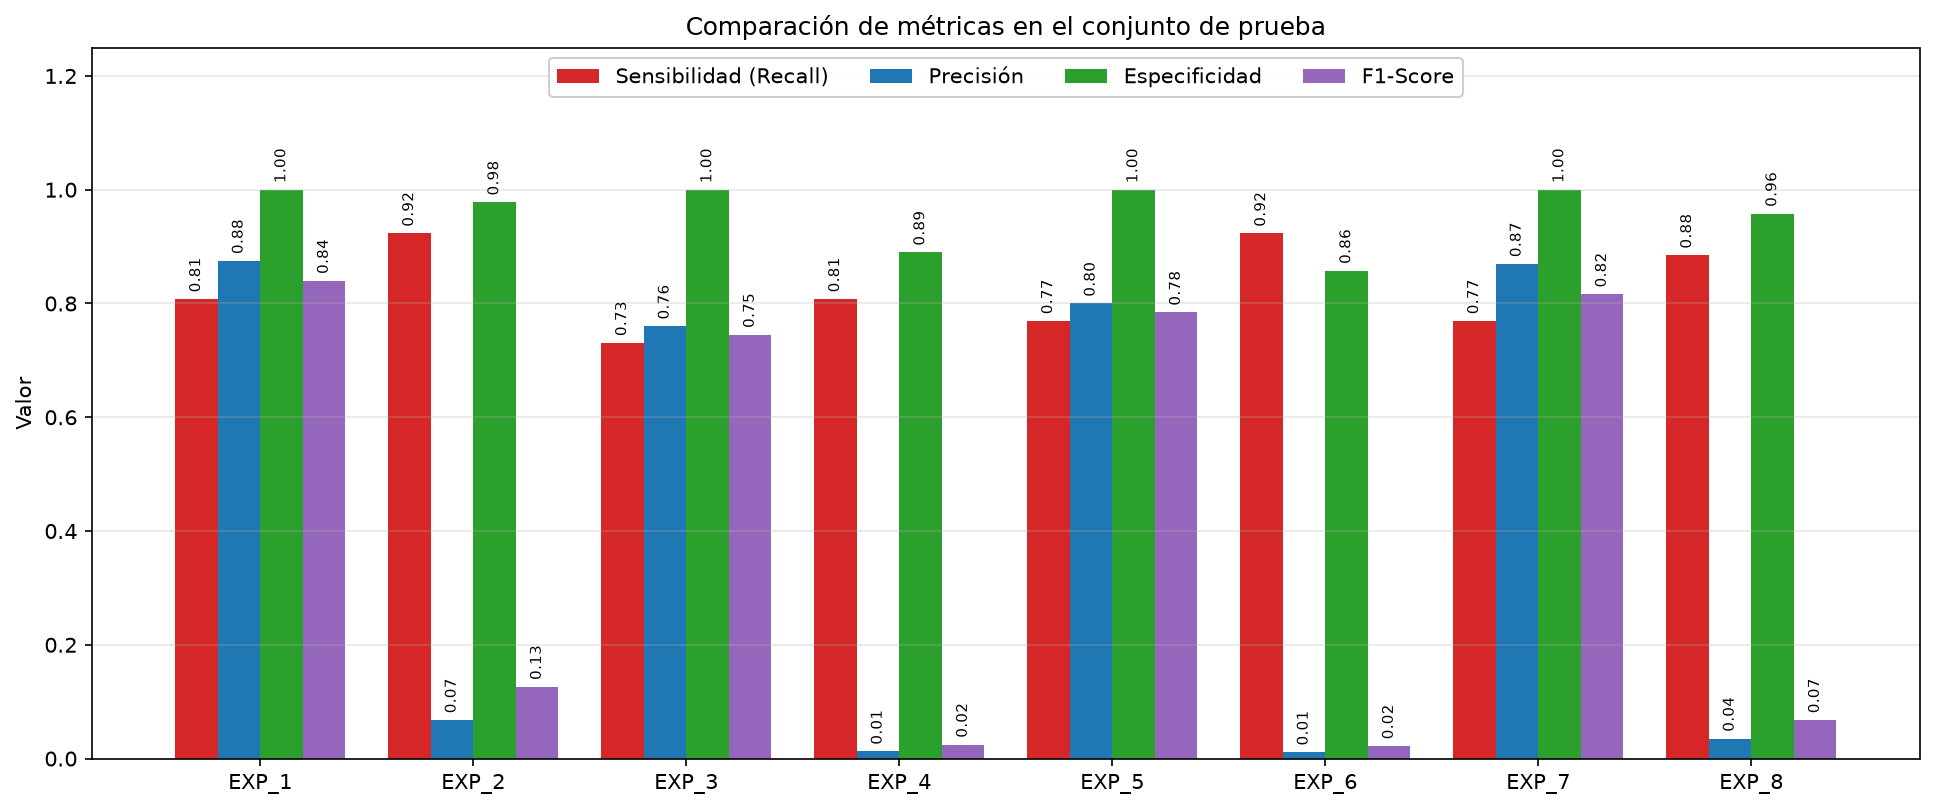
\includegraphics[width=\linewidth]{Graficos/comparacion_metricas.png}
    \end{column}
    \begin{column}{0.36\textwidth}
      \begin{block}{Hallazgos}
        \scriptsize
        \begin{itemize}
          \item La compensación sube el Recall y hunde la Precisión.
          \item Los FP crecen de 3 a 330 (k-NN), de 5 a 2.131 (SVM)
                y de 3 a 629 (RF).
          \item La exactitud sigue alta, pero el coste operativo de las
                falsas alarmas es enorme.
          \item Si el coste de un FP importa, EXP\_1 es la opción más
                equilibrada; si se prioriza Recall, EXP\_2 es preferible
                a EXP\_6 en prueba.
        \end{itemize}
      \end{block}
    \end{column}
  \end{columns}

  \vspace{0.1cm}
  \begin{alertblock}{Lectura}
    \small
    El mejor modelo depende del coste relativo de un FN frente a un FP;
    el criterio Recall-first no es suficiente por sí solo.
  \end{alertblock}
\end{frame}

% =====================================================================
% 10. ANÁLISIS CRÍTICO
% =====================================================================
\section{Análisis y conclusiones}

\begin{frame}{Análisis crítico}
  \begin{columns}[T]
    \begin{column}{0.49\textwidth}
      \begin{block}{Compensar el desbalance}
        \scriptsize
        \begin{itemize}
          \item Recall: +7,7 a +15,4 puntos porcentuales.
          \item FP: \(\times 110\) a \(\times 426\).
          \item Precisión: caída relativa de entre 92\,\% y 99\,\%.
          \item Ejemplo: k-NN pasa de 3 FP a 330; SVM de 5 a 2.131.
        \end{itemize}
      \end{block}
      \begin{block}{Árbol vs.\ ensamble}
        \scriptsize
        \begin{itemize}
          \item Sin compensación: RF mejora Recall 0,731\(\to\)0,769,
                Precisión 0,760\(\to\)0,870 y F1 0,745\(\to\)0,816.
          \item Con compensación: 0,808\(\to\)0,885,
                0,013\(\to\)0,035 y 0,025\(\to\)0,068.
          \item El bagging reduce varianza; el subespacio decorrelaciona.
        \end{itemize}
      \end{block}
    \end{column}
    \begin{column}{0.49\textwidth}
      \begin{block}{Fraudes detectados y falsas alarmas}
        \scriptsize
        \begin{itemize}
          \item k-NN + under: 24 TP, 2 FN, 330 FP.
          \item SVM + under: 24 TP, 2 FN, 2.131 FP.
          \item RF + under: 23 TP, 3 FN, 629 FP.
          \item Más Recall no implica mejor modelo: el coste de los FP
                puede superar el beneficio.
        \end{itemize}
      \end{block}
      \begin{block}{La exactitud engaña}
        \scriptsize
        \begin{itemize}
          \item Todo legítimo: 99,83\,\% de exactitud, 0\,\% de Recall.
          \item Todo fraude: 100\,\% de Recall, 0,1733\,\% de Precisión.
          \item La exactitud no distingue FP de FN ni refleja el coste.
        \end{itemize}
      \end{block}
    \end{column}
  \end{columns}
\end{frame}

% =====================================================================
% 11. CONCLUSIONES Y LIMITACIONES
% =====================================================================
\begin{frame}{Conclusiones y limitaciones}
  \begin{columns}[T]
    \begin{column}{0.49\textwidth}
      \begin{block}{Conclusiones y aprendizajes}
        \scriptsize
        \begin{itemize}
          \item Configuración seleccionada por CV: EXP\_6 (SVM + under),
                Recall CV 0,950 \(\pm\) 0,041.
          \item En prueba: Recall 0,923; Precisión 0,011; F1 0,022;
                2 FN y 2.131 FP.
          \item EXP\_2 empata en Recall (0,923) con mejor Precisión/F1
                (0,068/0,126).
          \item EXP\_1 es el mejor equilibrio global: Precisión 0,875
                y F1 0,840.
          \item El RF propio mejora al árbol y supera al SVM en
                Precisión/F1, pero no alcanza el Recall de k-NN/SVM
                con compensación.
          \item La compensación mejora el Recall a costa de multiplicar
                las falsas alarmas; la exactitud sola es engañosa.
        \end{itemize}
      \end{block}
    \end{column}
    \begin{column}{0.49\textwidth}
      \begin{block}{Limitaciones}
        \scriptsize
        \begin{itemize}
          \item Muestra de 50.000 transacciones; solo 26 fraudes en test
                y alta varianza.
          \item Split aleatorio, no temporal; variables PCA y solo dos días.
          \item Criterio Recall-first sin coste explícito de FP.
          \item Sin PR-AUC, intervalos de confianza ni tests estadísticos.
          \item Submuestreo descarta datos; \texttt{LinearSVC} sin
                probabilidades calibradas; RF sin OOB.
        \end{itemize}
      \end{block}
      \begin{block}{Mejoras}
        \scriptsize
        \begin{itemize}
          \item Ejecutar el dataset completo y validación temporal.
          \item Añadir PR-AUC, calibración y umbral por coste.
          \item Comparar SMOTE, submuestreo y \texttt{class\_weight}.
          \item Analizar importancia de variables y estabilidad.
        \end{itemize}
      \end{block}
    \end{column}
  \end{columns}
\end{frame}

% =====================================================================
% 12. CIERRE
% =====================================================================
\begin{frame}
  \centering
  \Huge \textbf{Gracias}\\[0.4cm]
  \Large ¿Preguntas?
\end{frame}

% =====================================================================
% DIAPOSITIVAS DE RESPALDO
% =====================================================================
\appendix

\begin{frame}{Respaldo: resultados completos en prueba}
  \scriptsize
  \setlength{\tabcolsep}{2pt}
  \renewcommand{\arraystretch}{1.08}
  \begin{columns}[T]
    \begin{column}{0.58\textwidth}
      \resizebox{\linewidth}{!}{%
      \begin{tabular}{@{}l c c c c c c@{}}
        \toprule
        \textbf{ID} & \textbf{Recall} & \textbf{Prec.} & \textbf{Espec.} &
        \textbf{F1} & \textbf{Exact.} & \textbf{FNR} \\
        \midrule
        EXP\_1 & 0.808 & 0.875 & 0.9998 & 0.840 & 0.9995 & 0.192 \\
        EXP\_2 & 0.923 & 0.068 & 0.9780 & 0.126 & 0.9779 & 0.077 \\
        EXP\_3 & 0.731 & 0.760 & 0.9996 & 0.745 & 0.9991 & 0.269 \\
        EXP\_4 & 0.808 & 0.013 & 0.8898 & 0.025 & 0.8897 & 0.192 \\
        EXP\_5 & 0.769 & 0.800 & 0.9997 & 0.784 & 0.9993 & 0.231 \\
        EXP\_6 & 0.923 & 0.011 & 0.8577 & 0.022 & 0.8578 & 0.077 \\
        EXP\_7 & 0.769 & 0.870 & 0.9998 & 0.816 & 0.9994 & 0.231 \\
        EXP\_8 & 0.885 & 0.035 & 0.9580 & 0.068 & 0.9579 & 0.115 \\
        \bottomrule
      \end{tabular}%
      }
    \end{column}
    \begin{column}{0.40\textwidth}
      \resizebox{\linewidth}{!}{%
      \begin{tabular}{@{}l c c@{}}
        \toprule
        \textbf{ID} & \textbf{TP/FN/FP/TN} & \textbf{CV Recall} \\
        \midrule
        EXP\_1 & 21/5/3/14.971 & \(0.850 \pm 0.122\) \\
        EXP\_2 & 24/2/330/14.644 & \(0.900 \pm 0.062\) \\
        EXP\_3 & 19/7/6/14.968 & \(0.733 \pm 0.097\) \\
        EXP\_4 & 21/5/1.650/13.324 & \(0.900 \pm 0.122\) \\
        EXP\_5 & 20/6/5/14.969 & \(0.750 \pm 0.075\) \\
        EXP\_6 & 24/2/2.131/12.843 & \(0.950 \pm 0.041\) \\
        EXP\_7 & 20/6/3/14.971 & \(0.767 \pm 0.097\) \\
        EXP\_8 & 23/3/629/14.345 & \(0.917 \pm 0.053\) \\
        \bottomrule
      \end{tabular}%
      }
    \end{column}
  \end{columns}
  \vspace{0.1cm}
  {\scriptsize IDs: EXP\_1/2 k-NN; EXP\_3/4 Árbol; EXP\_5/6 SVM;
  EXP\_7/8 Random Forest propio.}
\end{frame}

\begin{frame}{Respaldo: matrices de confusión}
  \centering
  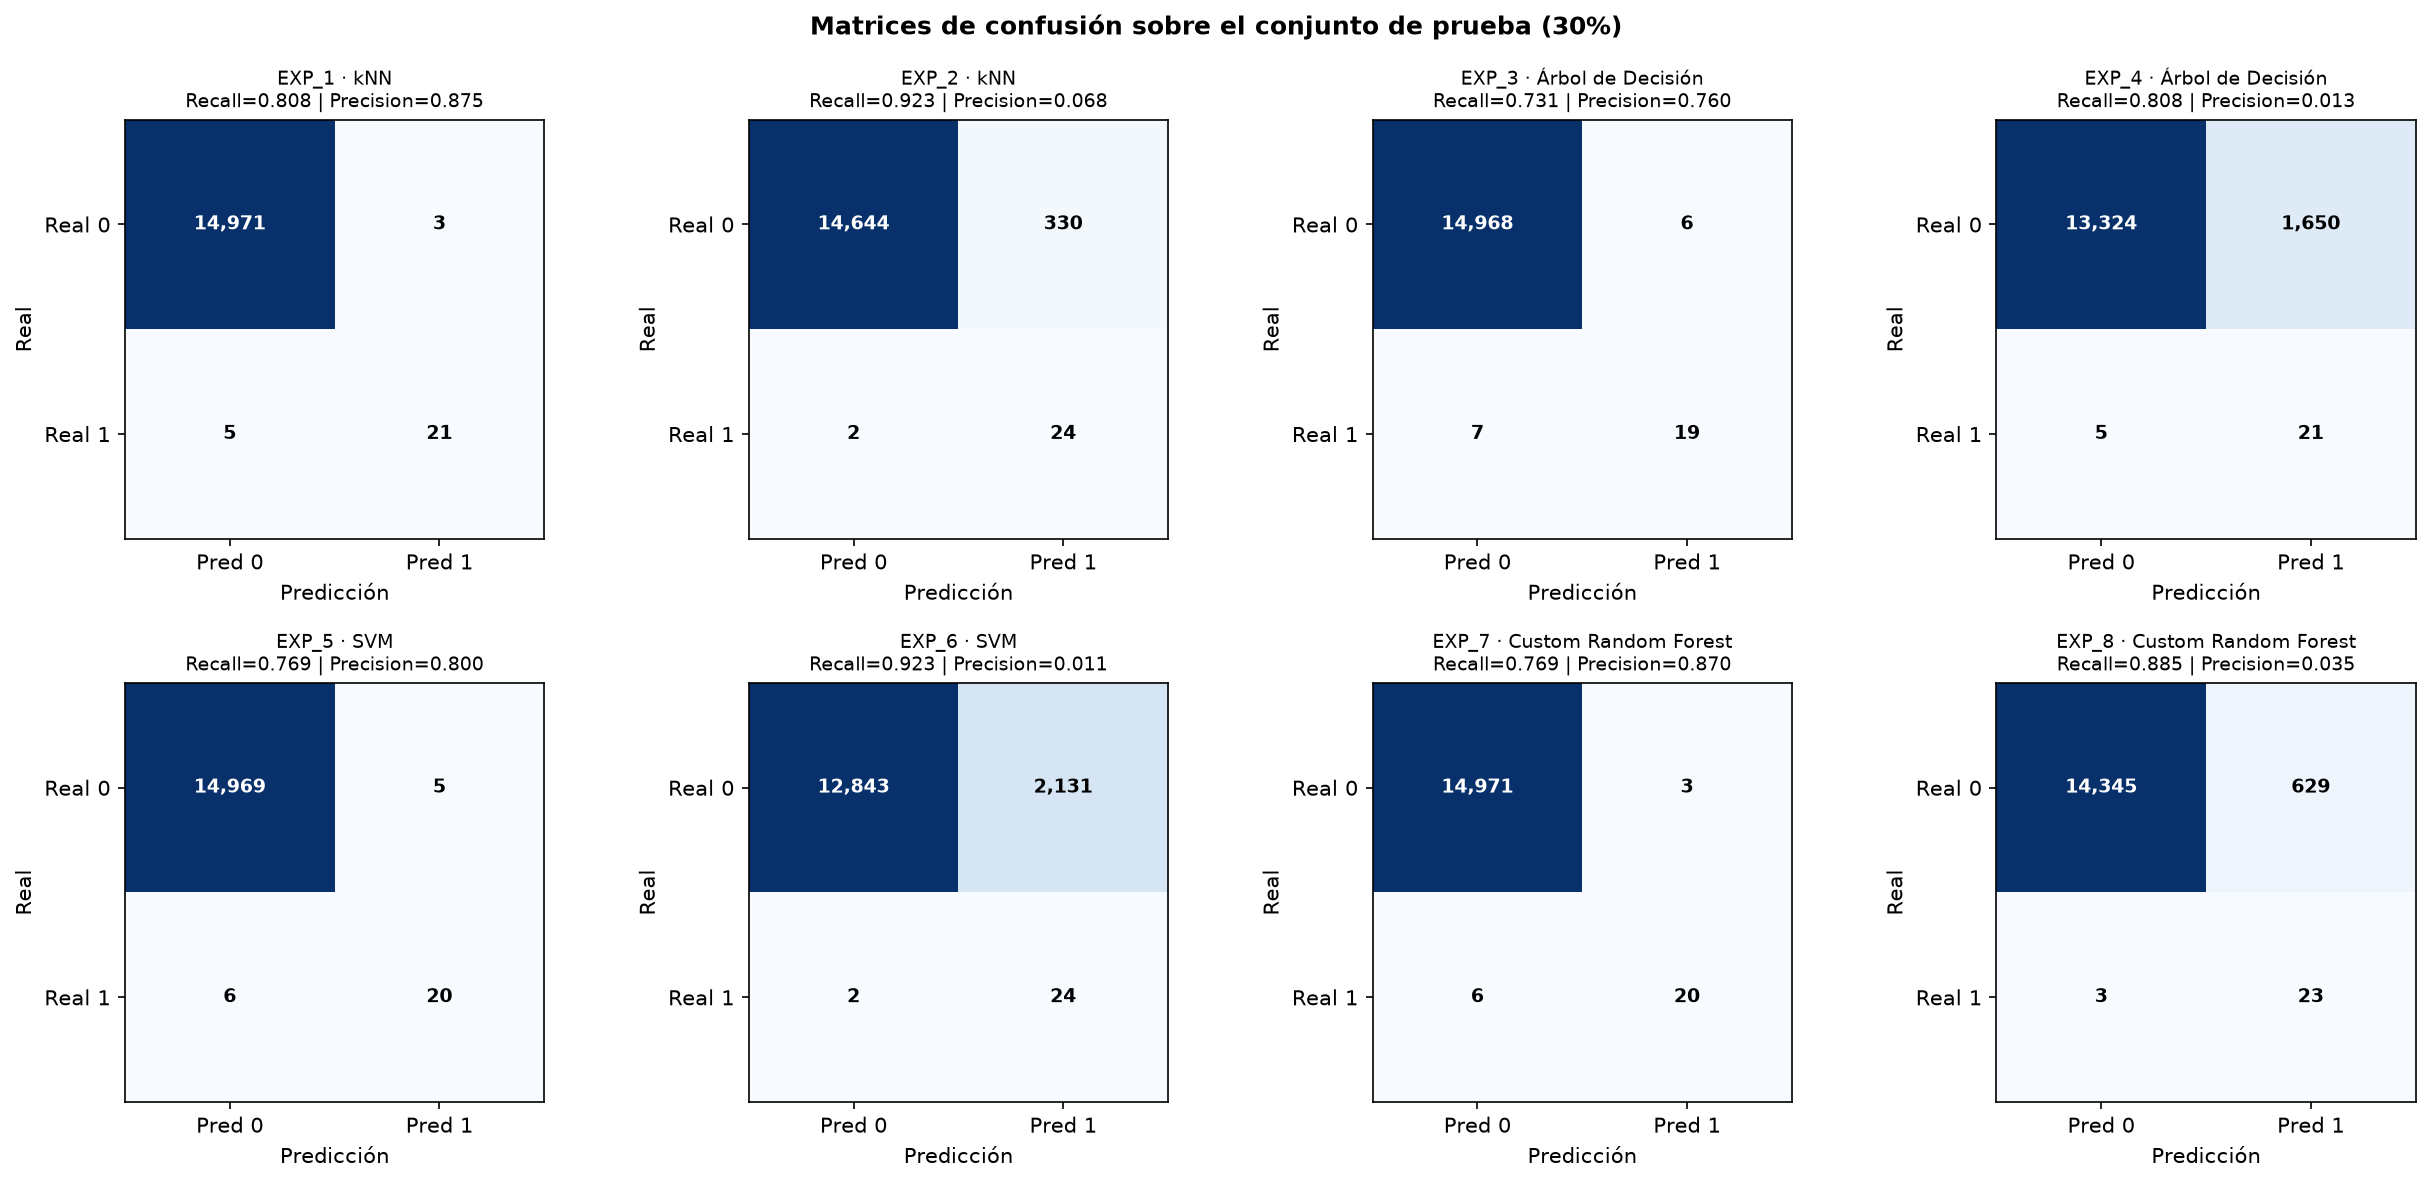
\includegraphics[width=0.95\textwidth,height=0.82\textheight,keepaspectratio]{Graficos/matrices_confusion.png}
\end{frame}

\begin{frame}{Respaldo: comparación de métricas}
  \centering
  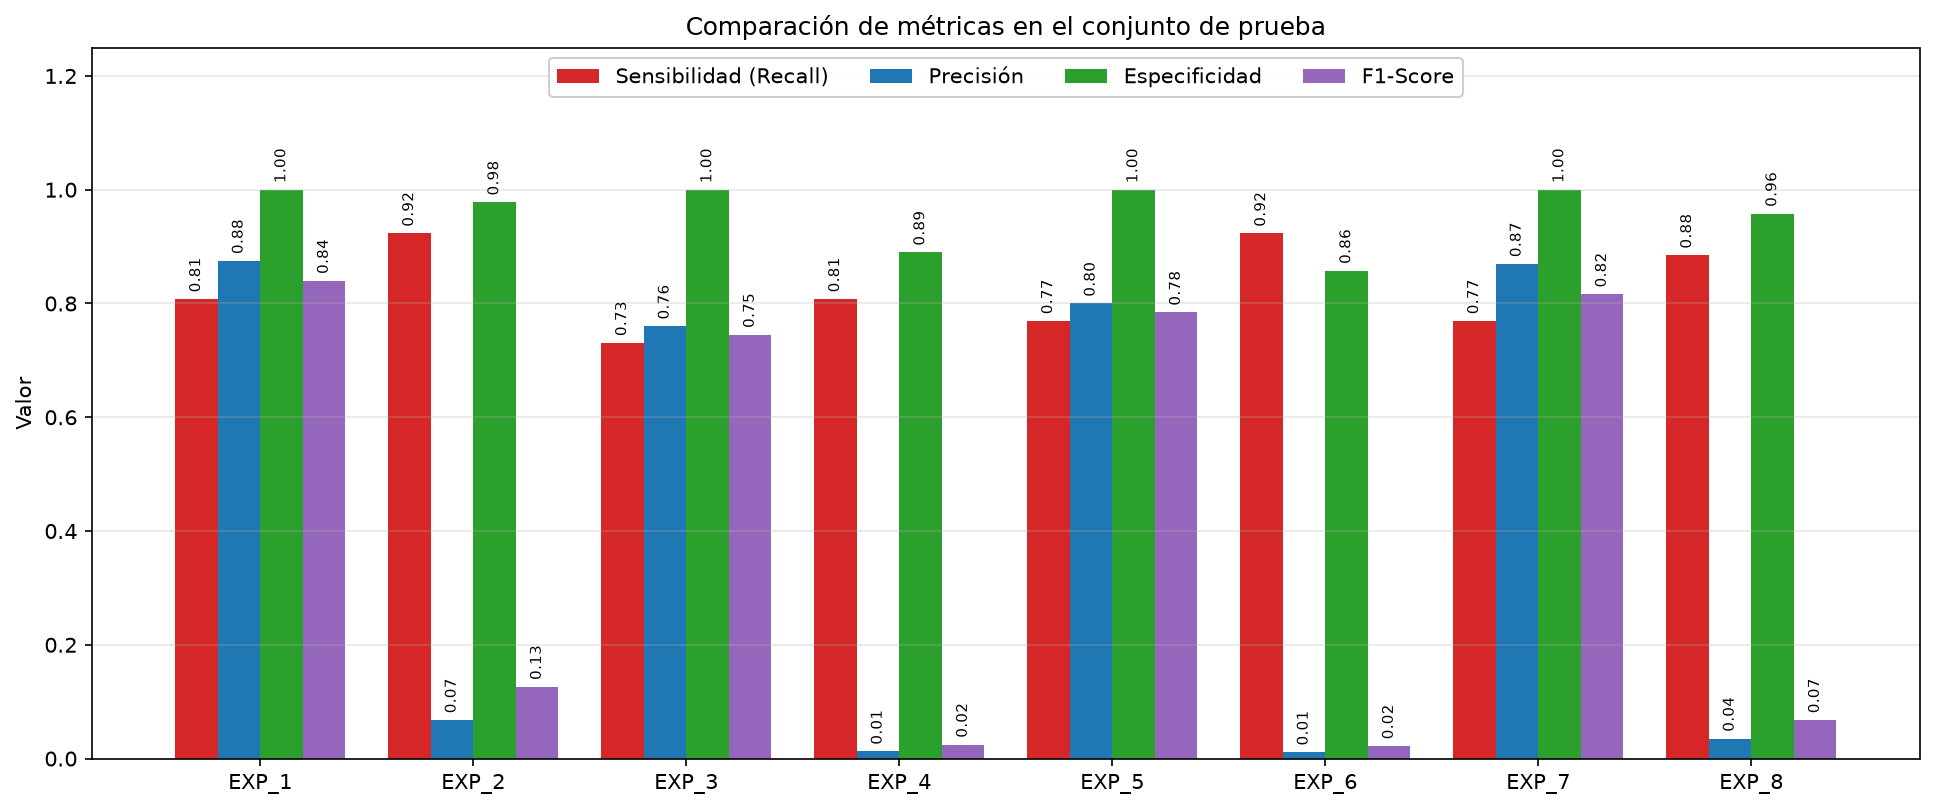
\includegraphics[width=0.95\textwidth,height=0.82\textheight,keepaspectratio]{Graficos/comparacion_metricas.png}
\end{frame}

\begin{frame}{Respaldo: Recall en validación cruzada}
  \centering
  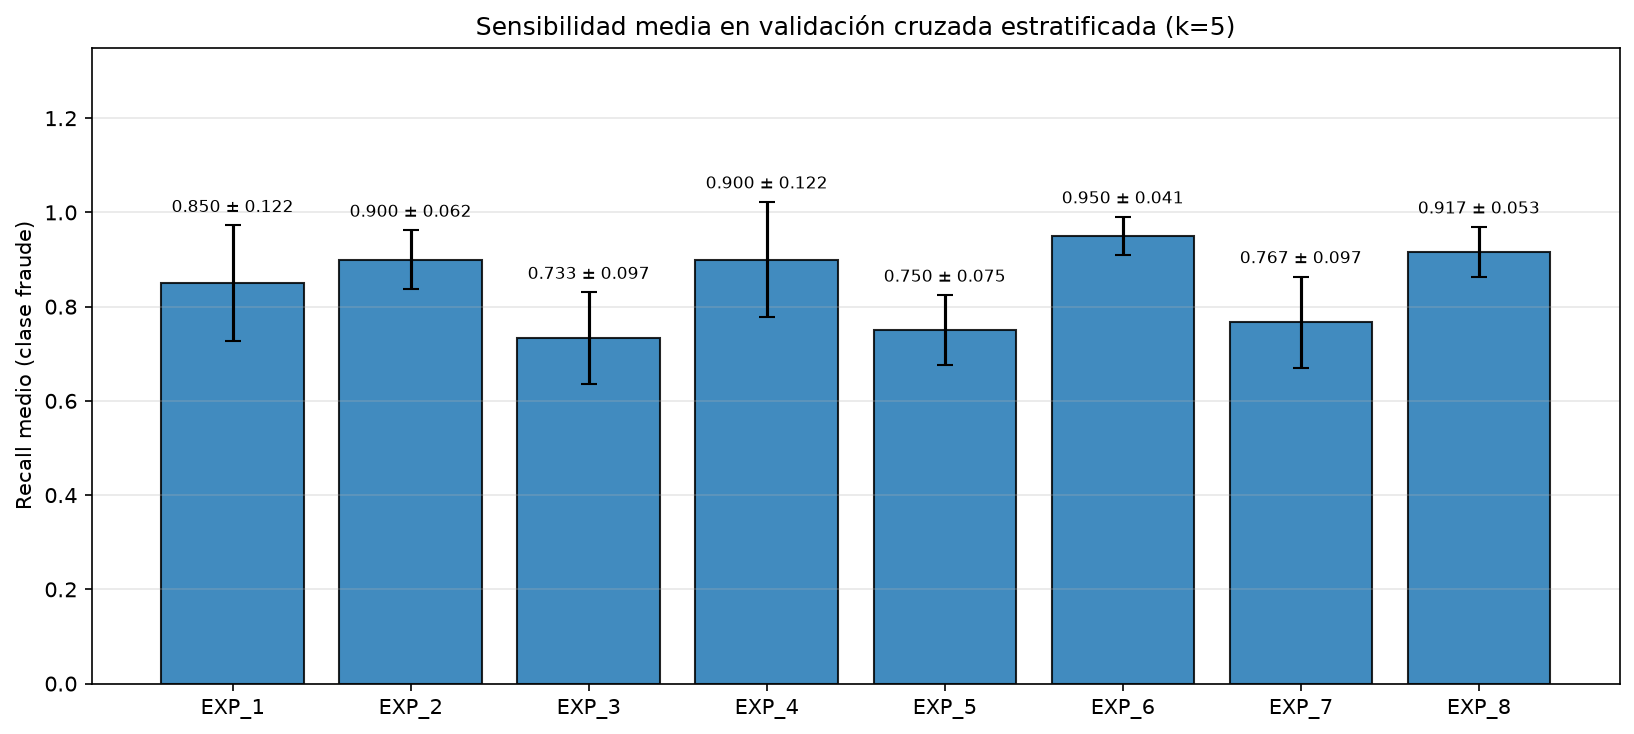
\includegraphics[width=0.95\textwidth,height=0.82\textheight,keepaspectratio]{Graficos/recall_validacion_cruzada.png}
\end{frame}

% ---------------------------------------------------------------------
\begin{frame}{Respaldo: exactitud y desbalanceo}
  \begin{columns}[T]
    \begin{column}{0.46\textwidth}
      \begin{block}{Clasificador trivial: todo legítimo}
        \scriptsize
        \begin{tabular}{@{}lr@{}}
          \toprule
          Métrica & Valor \\
          \midrule
          Exactitud & \textbf{99,8267\,\%} \\
          Sensibilidad (Recall) & \textbf{0\,\%} \\
          FNR & 100\,\% \\
          Especificidad & 100\,\% \\
          Precisión & no definida \\
          \bottomrule
        \end{tabular}
      \end{block}
      \vspace{0.1cm}
      {\scriptsize En la prueba hay 26 fraudes entre 15.000
      transacciones (0,1733\,\%).}
    \end{column}
    \begin{column}{0.50\textwidth}
      \begin{block}{Por qué la exactitud engaña}
        \scriptsize
        \begin{itemize}
          \item La exactitud está dominada por la clase mayoritaria.
          \item Un modelo que no detecta ningún fraude parece casi
                perfecto (99,83\,\%).
          \item No distingue el coste de un falso negativo del de un
                falso positivo.
          \item En fraude, los FN suelen ser mucho más costosos.
        \end{itemize}
      \end{block}
    \end{column}
  \end{columns}
  \vspace{0.15cm}
  \begin{alertblock}{Consecuencia}
    \small
    Hay que reportar Recall, FNR, Precisión, F1 y, si es posible,
    PR-AUC y coste económico; la exactitud sola no es un criterio
    válido con este desbalanceo.
  \end{alertblock}
\end{frame}

% ---------------------------------------------------------------------
\begin{frame}{Respaldo: efecto de la compensación}
  \scriptsize
  \setlength{\tabcolsep}{3pt}
  \renewcommand{\arraystretch}{1.15}
  \resizebox{\textwidth}{!}{%
  \begin{tabular}{@{}lccc@{}}
    \toprule
    \textbf{Modelo} & \textbf{Recall (sin $\to$ con)} &
    \textbf{Precisión (sin $\to$ con)} & \textbf{FP (sin $\to$ con)} \\
    \midrule
    k-NN   & 0,808 $\to$ \textbf{0,923} & \textbf{0,875} $\to$ 0,068 & 3 $\to$ \textbf{330} \\
    Árbol  & 0,731 $\to$ 0,808 & 0,760 $\to$ 0,013 & 6 $\to$ 1.650 \\
    SVM    & 0,769 $\to$ \textbf{0,923} & 0,800 $\to$ 0,011 & 5 $\to$ 2.131 \\
    RF     & 0,769 $\to$ 0,885 & 0,870 $\to$ 0,035 & 3 $\to$ 629 \\
    \bottomrule
  \end{tabular}%
  }
  \vspace{0.15cm}
  \begin{columns}[T]
    \begin{column}{0.49\textwidth}
      \begin{block}{Qué mejora}
        \scriptsize
        \begin{itemize}
          \item El Recall sube entre 7,7 y 15,4 puntos porcentuales.
          \item Los FN bajan: por ejemplo, k-NN pasa de 5 a 2.
          \item Se detectan más fraudes con el mismo umbral.
        \end{itemize}
      \end{block}
    \end{column}
    \begin{column}{0.49\textwidth}
      \begin{block}{Qué empeora}
        \scriptsize
        \begin{itemize}
          \item Los FP se multiplican entre 110\(\times\) y 426\(\times\).
          \item La Precisión cae entre 92\,\% y 99\,\% (relativo).
          \item La exactitud sigue alta, pero el modelo es
                operativamente agresivo.
        \end{itemize}
      \end{block}
    \end{column}
  \end{columns}
  \vspace{0.1cm}
  \begin{alertblock}{Lectura}
    \small
    Compensar mejora la sensibilidad, pero traslada el coste a las
    falsas alarmas. La decisión depende del coste de un FN frente al
    de un FP.
  \end{alertblock}
\end{frame}

% ---------------------------------------------------------------------
\begin{frame}{Respaldo: árbol individual vs.\ Random Forest}
  \scriptsize
  \setlength{\tabcolsep}{3pt}
  \renewcommand{\arraystretch}{1.15}
  \resizebox{\textwidth}{!}{%
  \begin{tabular}{@{}llccccc@{}}
    \toprule
    \textbf{Escenario} & \textbf{Modelo} & \textbf{Recall} &
    \textbf{Precisión} & \textbf{F1} & \textbf{FP} & \textbf{FN} \\
    \midrule
    Sin comp. & Árbol     & 0,731 & 0,760 & 0,745 & 6 & 7 \\
    Sin comp. & RF propio & \textbf{0,769} & \textbf{0,870} & \textbf{0,816} & \textbf{3} & \textbf{6} \\
    Con comp. & Árbol     & 0,808 & 0,013 & 0,025 & 1.650 & 5 \\
    Con comp. & RF propio & \textbf{0,885} & \textbf{0,035} & \textbf{0,068} & \textbf{629} & \textbf{3} \\
    \bottomrule
  \end{tabular}%
  }
  \vspace{0.15cm}
  \begin{columns}[T]
    \begin{column}{0.49\textwidth}
      \begin{block}{Qué aporta la combinación}
        \scriptsize
        \begin{itemize}
          \item \textbf{Bagging}: promedia árboles entrenados con
                muestras bootstrap y reduce la varianza.
          \item \textbf{Subespacio aleatorio}: decorrelaciona los
                árboles al limitar las variables por división.
          \item \textbf{Votación}: hace la predicción más robusta
                frente a ruido y valores atípicos.
        \end{itemize}
      \end{block}
    \end{column}
    \begin{column}{0.49\textwidth}
      \begin{block}{Efecto observado}
        \scriptsize
        \begin{itemize}
          \item Mejora Recall, Precisión y F1 frente al árbol.
          \item Reduce FP (6\(\to\)3 y 1.650\(\to\)629) y FN.
          \item En CV con compensación: 0,917 \(\pm\) 0,053 frente a
                0,900 \(\pm\) 0,122 del árbol (más estable).
          \item No elimina el sesgo por desbalanceo: con submuestreo
                siguen apareciendo muchas falsas alarmas.
        \end{itemize}
      \end{block}
    \end{column}
  \end{columns}
\end{frame}

% ---------------------------------------------------------------------
\begin{frame}{Respaldo: configuración seleccionada por CV}
  \begin{columns}[T]
    \begin{column}{0.48\textwidth}
      \begin{block}{EXP\_6: SVM lineal + submuestreo}
        \scriptsize
        \begin{itemize}
          \item Mejores hiperparámetros:
                \texttt{select\_k=all}, \(C=0.1\).
          \item Recall CV: \textbf{0,950 \(\pm\) 0,041}.
          \item Precisión CV: 0,018 \(\pm\) 0,002.
        \end{itemize}
      \end{block}
      \vspace{0.1cm}
      \begin{block}{Desempeño en prueba}
        \scriptsize
        \begin{tabular}{@{}lr@{}}
          \toprule
          Métrica & Valor \\
          \midrule
          Recall & \textbf{92,31\,\%} (24/26) \\
          Precisión & \textbf{1,11\,\%} \\
          Especificidad & 85,77\,\% \\
          F1 & 2,20\,\% \\
          Exactitud & 85,78\,\% \\
          FNR & 7,69\,\% \\
          TP / FN / FP / TN & 24 / 2 / 2.131 / 12.843 \\
          \bottomrule
        \end{tabular}
      \end{block}
    \end{column}
    \begin{column}{0.48\textwidth}
      \begin{block}{Contexto y cautela}
        \scriptsize
        \begin{itemize}
          \item Solo hay 26 fraudes en prueba: un fraude vale
                3,85 pp de Recall.
          \item EXP\_8 (RF + under): Recall CV 0,917; en prueba
                88,5\,\% con Precisión 3,53\,\% y F1 6,78\,\%
                (629 FP).
          \item EXP\_2 (k-NN + under): mismo Recall en prueba
                (92,31\,\%) con Precisión 6,78\,\% y F1 12,63\,\%.
          \item Si el coste de un FP importa, EXP\_2/EXP\_8 pueden
                ser preferibles a la ganadora por Recall puro.
        \end{itemize}
      \end{block}
    \end{column}
  \end{columns}
  \vspace{0.1cm}
  \begin{alertblock}{Interpretación}
    \small
    EXP\_6 es la mejor por el criterio CV (Recall), pero no es
    necesariamente la mejor opción operativa: su Precisión es muy baja.
  \end{alertblock}
\end{frame}

% ---------------------------------------------------------------------
\begin{frame}{Respaldo: limitaciones y clasificador ``todo fraude''}
  \begin{columns}[T]
    \begin{column}{0.54\textwidth}
      \begin{block}{Limitaciones}
        \scriptsize
        \begin{itemize}
          \item Muestra de 50.000 transacciones; solo 26 fraudes en
                prueba y alta varianza (desviaciones CV de 4--12 pp).
          \item Split aleatorio, no temporal; variables PCA y solo dos
                días de transacciones.
          \item El criterio Recall-first ignora el coste de los FP;
                faltan PR-AUC, intervalos de confianza y tests.
          \item El submuestreo descarta la mayoría de las legítimas;
                \texttt{LinearSVC} no da probabilidades calibradas y el
                RF propio no tiene OOB ni poda.
          \item Sin contexto de cliente o comercio; no se evalúan
                equidad, latencia ni deriva.
        \end{itemize}
      \end{block}
    \end{column}
    \begin{column}{0.44\textwidth}
      \begin{block}{Clasificar todo como fraude}
        \scriptsize
        \begin{tabular}{@{}lr@{}}
          \toprule
          Métrica & Valor \\
          \midrule
          Recall & \textbf{100\,\%} \\
          Precisión & \textbf{0,1733\,\%} \\
          Especificidad & \textbf{0\,\%} \\
          F1 & 0,346\,\% \\
          Exactitud & 0,1733\,\% \\
          TP / FN / FP / TN & 26 / 0 / 14.974 / 0 \\
          \bottomrule
        \end{tabular}
      \end{block}
      \vspace{0.1cm}
      {\scriptsize \textbf{Consecuencia:} se detectan todos los fraudes,
      pero se bloquean 14.974 transacciones legítimas. El coste
      operativo y reputacional es inasumible.}
    \end{column}
  \end{columns}
  \vspace{0.15cm}
  \begin{alertblock}{Idea clave}
    \small
    El Recall por sí solo no basta: hay que analizar conjuntamente
    Precisión, FP y el coste de negocio de cada error.
  \end{alertblock}
\end{frame}

\end{document}
